% Time-stamp: <2025-03-13 10:50:40>


\documentclass[presentation,aspectratio=1610]{beamer}

%% Full theme: AnnArbor Antibes Bergen Berkeley Berlin Boadilla boxes CambridgeUS Copenhagen Darmstadt default Dresden EastLansing Frankfurt Goettingen Hannover Ilmenau JuanLesPins Luebeck Madrid Malmoe Marburg Montpellier PaloAlto Pittsburgh Rochester Singapore Szeged Warsaw
% \usetheme{Luebeck}

%% outer themes (header/footer): default infolines miniframes smoothbars sidebar split shadow tree smoothtree
% \useoutertheme[subsection=false]{smoothbars}
% \usetheme{Rochester}
 \useoutertheme{split}

%% inner theme (content): default circles rectangles rounded inmargin
\useinnertheme{rectangles}

\usecolortheme{beaver}

\input{style}



\defcolvar{n}{n}{red}
\defcolvar{m}{m}{purple}
\defcolvar{alpha}{\alpha}{red}
\defcolvar{S}{S}{darkgreen}
\defcolvar{x}{x}{darkgreen}
\defcolvar{y}{y}{darkgreen}
\defcolvar{q}{q}{red}

\title{Symmetric Techniques for Advanced Protocols: What *are* They?}
\author[Léo Perrin]{Léo Perrin\inst{1} }

\institute{Inria, Paris}
\titlegraphic{\includegraphics[height=1.1cm]{figures/inria}}


\date{14th of March 2025}




\begin{document}

{
  \pagestyle{empty}

  \maketitle


  \begin{frame}{Trendy topics}

    \begin{itemize}
      \large
    \item [] MPC-friendly? 
    \item [] Arithmetization-Oriented?
    \item [] Verification efficiency?
    \item [] Algebraic attacks? \pause
    \item [] Symmetric crypto \textbf{for the blockchain...} \pause
    \item [] \alert{... for neural networks???}
    \end{itemize}
    \begin{center}
      The conclusion of today: \textbf{symmetric cryptography} has always had to deal with specific \textbf{implementation criteria}, but the \alert{new ones} are indeed a bit \textbf{stranger than before}.
    \end{center}
  \end{frame}
}


\tocStartsAppearingHere{}


\section{What is the Purpose of a Symmetric Primitive}

\subsection{Let's look at primitives we all know}


\begin{frame}{Why do we need symmetric primitives?}
  \vfill

  \begin{center}
    \includegraphics[width=8cm]{./figures/simpsons}
  \end{center}
  
  \vfill
\end{frame}


\begin{frame}{Unstable Definitions}
  \begin{alertblock}{What is ``efficient'' varies}
    \begin{itemize}
    \item What are the operations that we \textbf{can} use?
    \item What are the associated \textbf{costs}? 
    \end{itemize}
    \begin{center}
      How to get the best security for a given price?
    \end{center}
  \end{alertblock}

  
  
  \begin{exampleblock}{What is ``secure'' varies}
    \begin{itemize}
    \item Should the primitive work in many context? \hfill\onslide<4>{Modularity vs. Single use}
    \item Do we care about nonce-misuse? \hfill\onslide<4>{Robustness vs. ``not our problem''}
    \end{itemize}
    \begin{center}
      How do we define the \textbf{security} that the primitive must provide?

      \vspace{0.3cm}\pause
      What are the relevant forms of cryptanalysis?
    \end{center}
  \end{exampleblock}
\end{frame}


\subsection{A Small Cog in a Big Machine}


\begin{frame}{Web Encryption}
  \begin{center}
    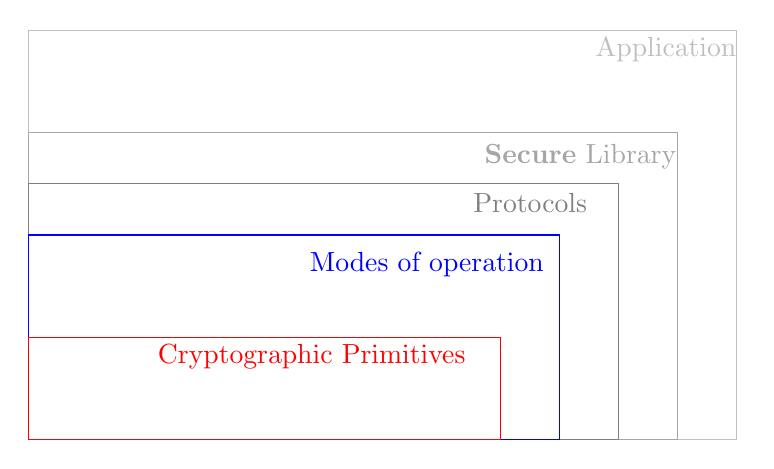
\begin{tikzpicture}[xscale=1.5,yscale=1.3]
      \draw[color=gray!50!white] (0, 0) rectangle (6, 4) node[pos=0.9,above] {Application};
      \onslide<2->{
        \draw[color=gray!70!white] (0, 0) rectangle (5.5, 3) node[pos=0.85,above] {\textbf{Secure} Library};
      }
      \onslide<3->{
        \draw[color=gray] (0, 0) rectangle (5, 2.5) node[pos=0.85,above] {Protocols};
      }
      \onslide<4->{
        \draw[color=blue] (0, 0) rectangle (4.5, 2) node[pos=0.75,above] {Modes of operation};
      }
      \onslide<5->{
        \draw[color=red] (0, 0) rectangle (4, 1) node[pos=0.6,above] {Cryptographic Primitives};
      }
    \end{tikzpicture}

    \begin{itemize}
    \item<6-> We want \alert{software efficient} (computer and smartphone but not micro-controllers) efficient \alert{AEAD} for packets of a few tens to a few billion bytes.
    \item<7> AES-GCM; Chacha-poly1305.
    \end{itemize}
  \end{center}
\end{frame}


\begin{frame}{What Chacha looks like}
  \begin{columns}
    \hfill
    \begin{column}{0.4\textwidth}
      \begin{center}
        \includegraphics[width=4cm]{./figures/chacha}
      \end{center}
    \end{column}
    \hfill
    \begin{column}{0.4\textwidth}
      \begin{itemize}
      \item Addition ~/~ Rotation ~/~ XOR
      \item 256-bit key
      \item 512-bit state
      \item Defined over 32-bit words
      \end{itemize}
    \end{column}
    \hfill
  \end{columns}
\end{frame}


\begin{frame}{RAM Encryption}
  \begin{center}
    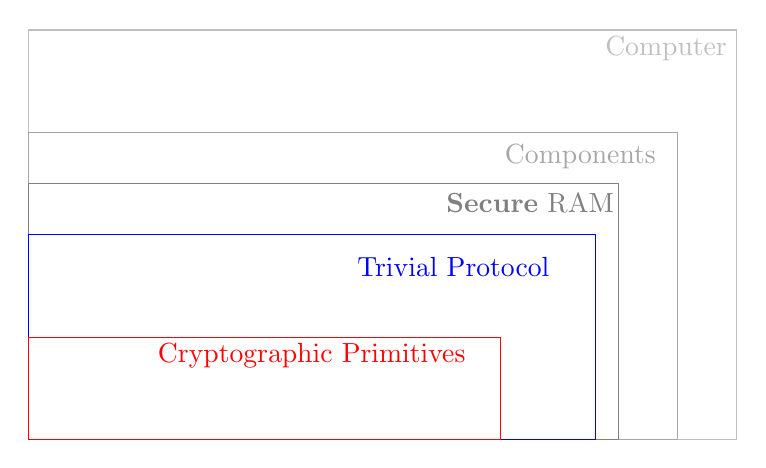
\begin{tikzpicture}[xscale=1.5,yscale=1.3]
      \draw[color=gray!50!white] (0, 0) rectangle (6, 4) node[pos=0.9,above] {Computer};
      \onslide<2->{
        \draw[color=gray!70!white] (0, 0) rectangle (5.5, 3) node[pos=0.85,above] {Components};
      }
      \onslide<3->{
        \draw[color=gray] (0, 0) rectangle (5, 2.5) node[pos=0.85,above] {\textbf{Secure} RAM};
      }
      \onslide<4->{
        \draw[color=blue] (0, 0) rectangle (4.8, 2) node[pos=0.75,above] {Trivial Protocol};
      }
      \onslide<5->{
        \draw[color=red] (0, 0) rectangle (4, 1) node[pos=0.6,above] {Cryptographic Primitives};
      }
    \end{tikzpicture}

    \begin{itemize}
    \item<6-> We want \alert{very low latency} \alert{block encryption} for specific (and small) block sizes.
    \item<7> PRINCE? QARMA? not so clear at this stage.
    \end{itemize}
  \end{center}
\end{frame}


\begin{frame}{What PRINCE looks like}
  \begin{center}
    \includegraphics[width=12cm]{./figures/prince}

    \begin{itemize}
    \item 4-bit S-box optimized for hardware
    \item 2 different matrices
    \item FX construction
    \item ``$\alpha$-reflexion''
    \item inverse rounds used in the second half
    \end{itemize}

  \end{center}
\end{frame}


\begin{frame}{Some Constants}
  \begin{itemize}
    \setlength\itemsep{1cm}
    \large
  \item A symmetric primitive is a very \alert{small} (but crucial) cog in a
    very big machine, \pause
  \item there are many \alert{different} ``big machines'', and \pause
  \item this has a \alert{huge influence} on what the primitive looks like.
  \end{itemize}
\end{frame}


\section{``Advanced'' Protocols}

\subsection{General Introduction}

\begin{frame}{Securing Data}
  \begin{center}
    {\Large Usually, we secure \alert{data} (at rest or in transit).}
    
    \only<1>{
\includegraphics[width=9cm]{./figures/crypto}}
    \only<2>{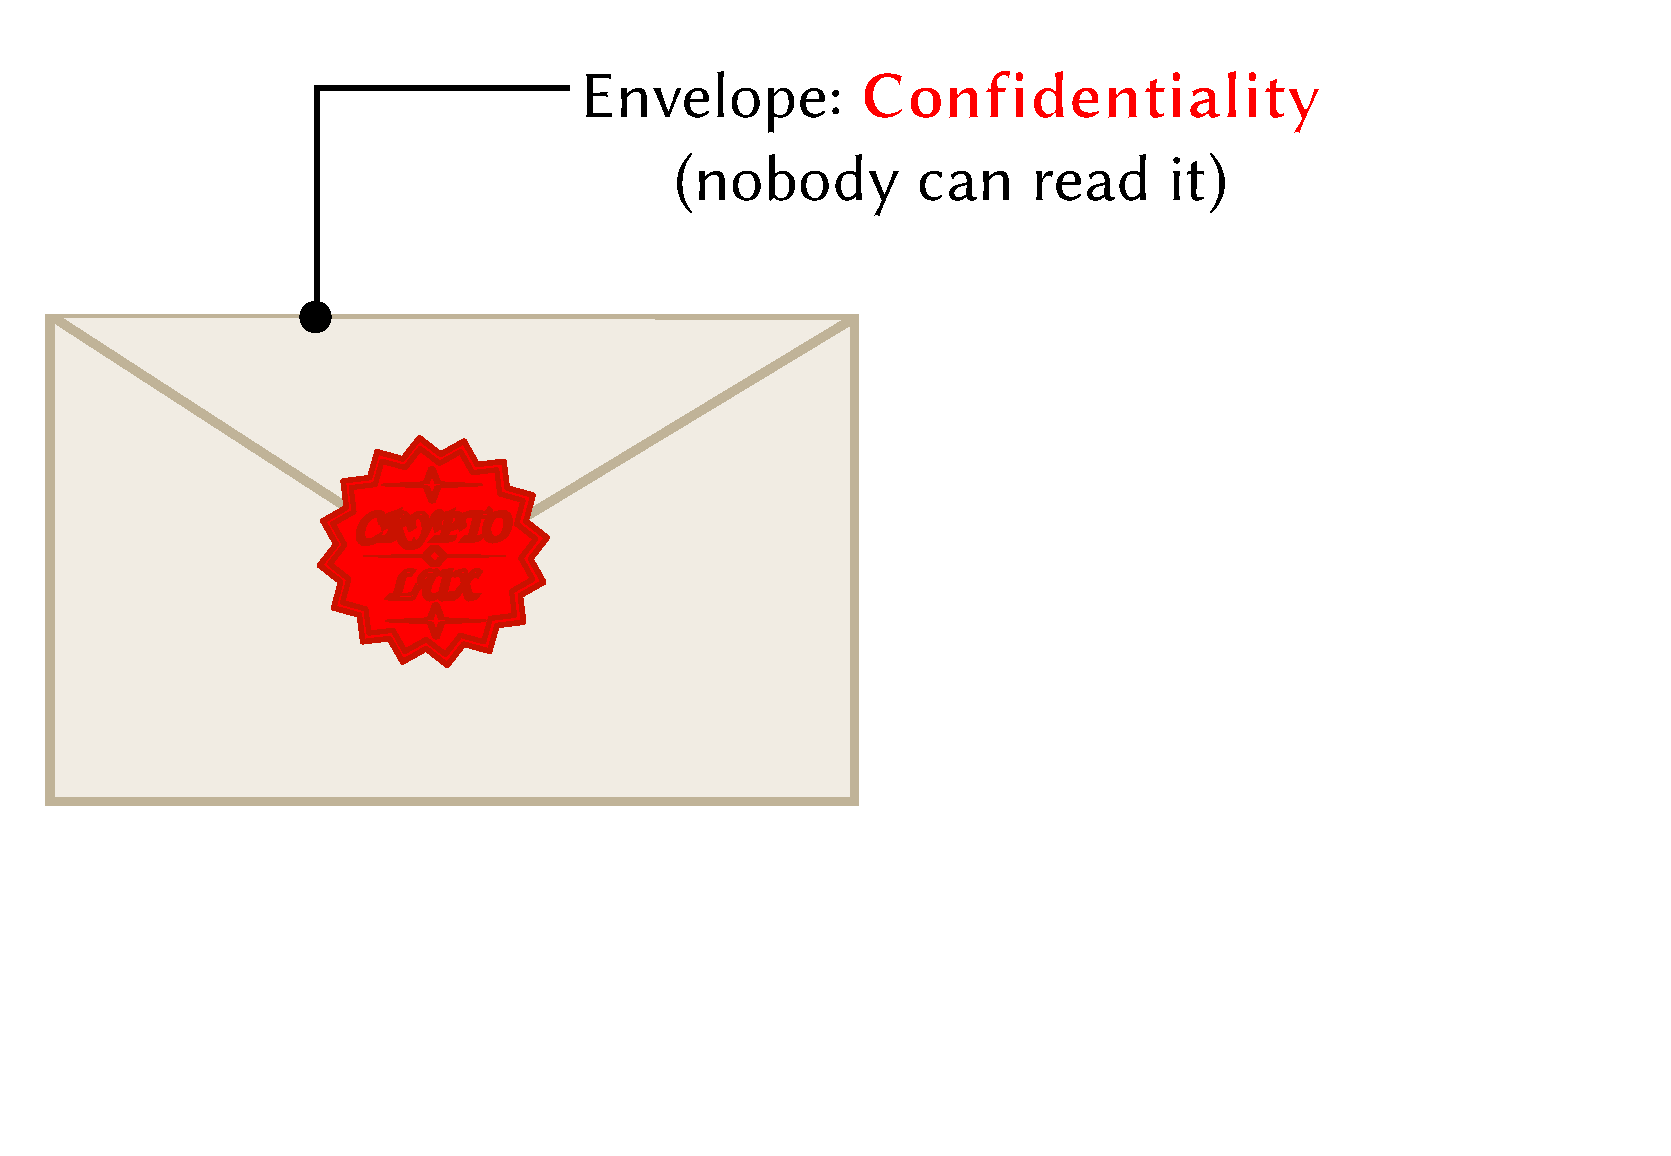
\includegraphics[width=9cm]{./figures/crypto-conf}}
    \only<3>{\includegraphics[width=9cm]{./figures/crypto-conf-int}}
    \only<4>{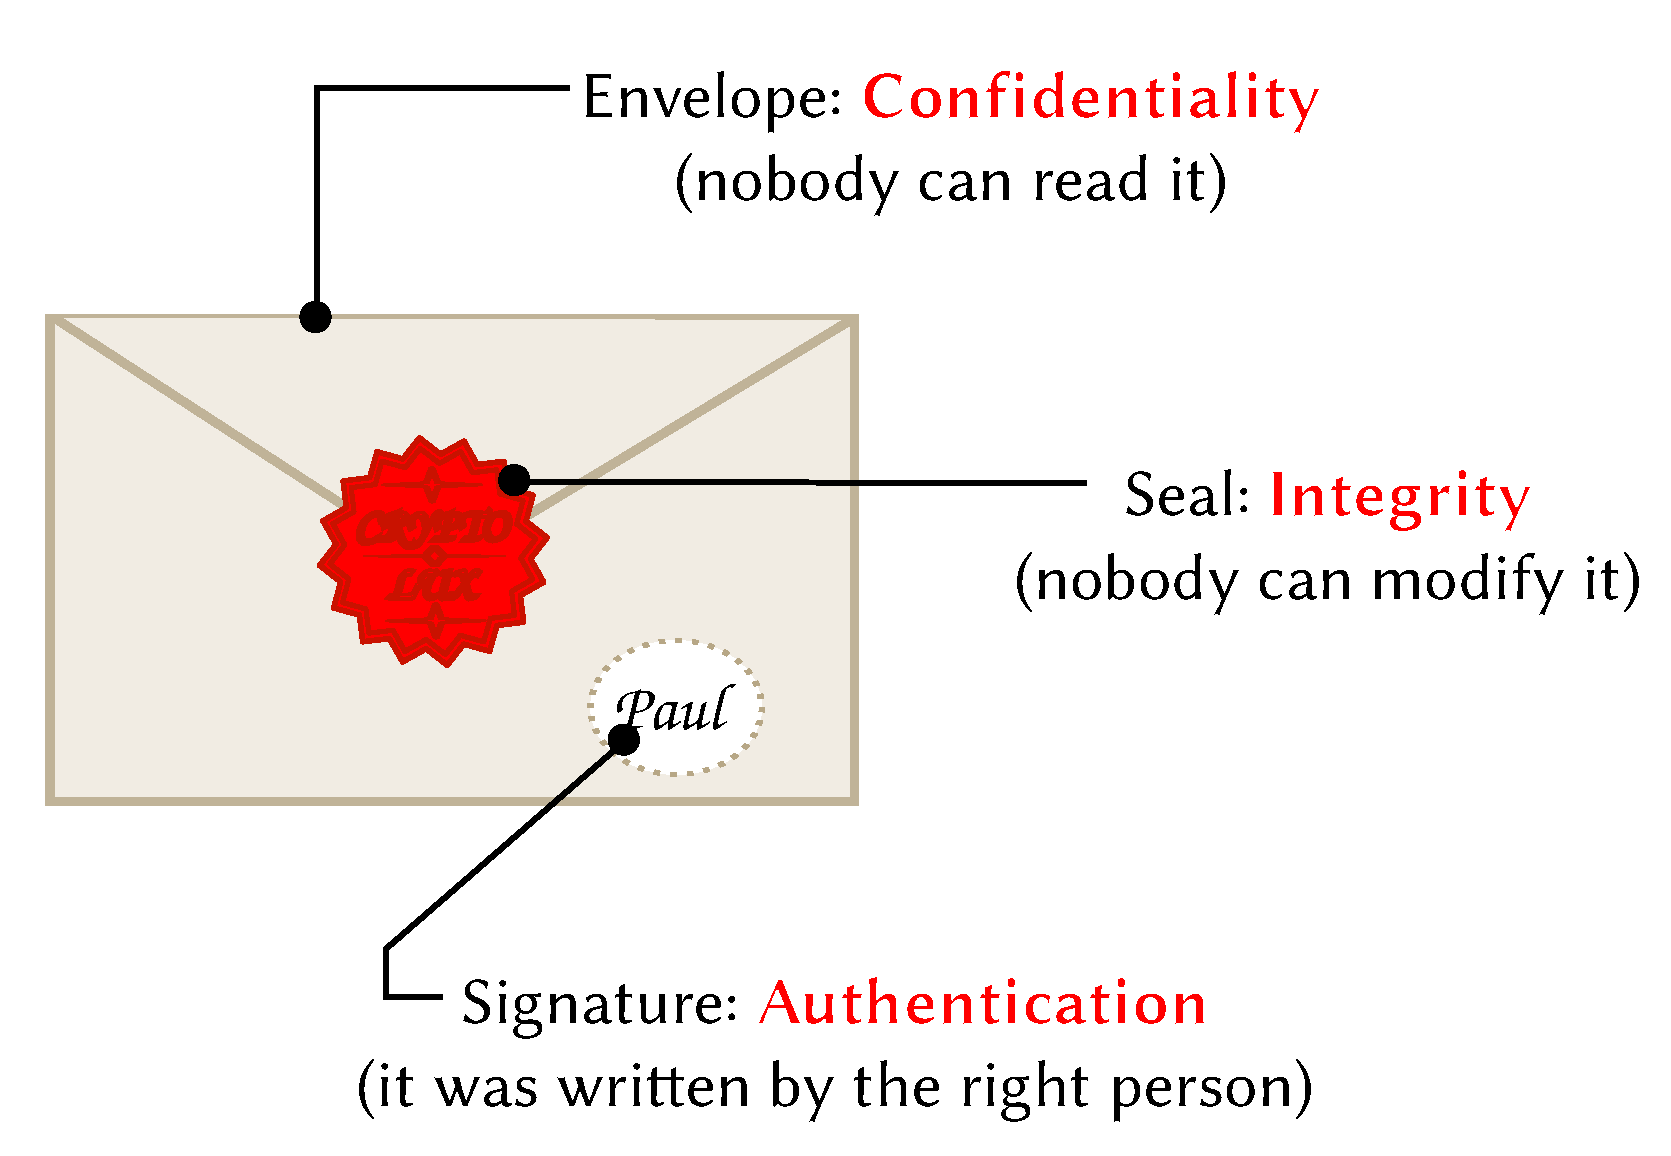
\includegraphics[width=9cm]{./figures/crypto-all}}
  \end{center}
\end{frame}


\begin{frame}{Securing Computation}
  \begin{center}
    {\Large More and more protocols intend to secure \alert{computations}.}

    \vspace{0.8cm}
    
    \begin{description}
    \item[FHE] \alert{F}ully \alert{H}omomorphic \alert{E}ncryption
    \item[MPC] \alert{M}ulti \alert{P}arty \alert{C}omputations
    \item[ZK-*] \alert{Z}ero \alert{K}nowledge- $[$ proof, argument... $]$
    \end{description}
  \end{center}
\end{frame}


\subsection{Different Protocols for Different Goals}

\begin{frame}{FHE}
  \begin{exampleblock}{Goal}
    Allow a third party to perform some operations on encrypted ciphertext that correspond to meaningful operations on the corresponding plaintext. \hfill \pause \alert{A form of commutation}    
  \end{exampleblock}

  \pause

  \begin{columns}
    \begin{column}{0.55\textwidth}
      \begin{center}
        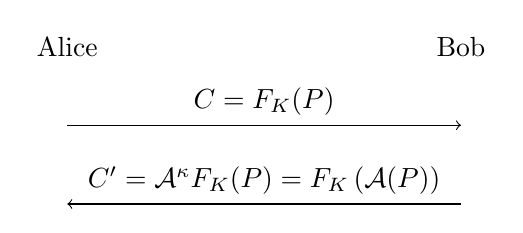
\begin{tikzpicture}
          \draw (0, 0) node(A){Alice} ;
          \draw (5, 0) node(B){Bob} ;
          \draw[->] (0, -1) -- (5, -1) node[pos=0.5,above]{$C = F_K(P)$};
          \draw[->] (5, -2) -- (0, -2) node[pos=0.5,above]{$C' = \mathcal{A}^{\kappa} F_K(P) = F_K\left(\mathcal{A}(P)\right)$};
        \end{tikzpicture}
      \end{center}
    \end{column}
    \begin{column}{0.4\textwidth}
      $F_K$ is a homomorphic cipher,

      \textbf{not} a block cipher!
    \end{column}
  \end{columns}

  \pause

  \begin{alertblock}{An example of (not F)HE}
    XOR-ing a constant to a ciphertext obtained using a stream cipher XORs the same constant in the plaintext:
    \begin{equation*}
      C \oplus t  = (P \oplus K) \oplus t = (P \oplus t) \oplus K
    \end{equation*}
  \end{alertblock}
\end{frame}


\begin{frame}{Multi-Party Computations}
  \begin{exampleblock}{Goal}
    Allow multiple parties to evaluate a function together even if some parties are not trustworthy.
  \end{exampleblock}

  \pause
  
  \begin{alertblock}{Example}
    Shamir's secret sharing
  \end{alertblock}

  \pause

  \begin{block}{Applications}
    \begin{itemize}
    \item Masking (the side-channel attack counter-measure)
    \item MPC-in-the-head paradigm (e.g. for Picnic signatures)
    \item ...
    \end{itemize}
  \end{block}
\end{frame}




\begin{frame}{Zero-Knowledge}
  \begin{exampleblock}{Principle}
    I want to convince you I know a secret \alert{without revealing it}
  \end{exampleblock}

  \pause
  \begin{block}{A generic goal}
    To be able to prove/argue that a function was evaluated correctly
    without revealing its input.

    \pause

    Ex: Sudoku time!
  \end{block}


  \pause
  
  \begin{block}{Applications}
    \begin{itemize}
    \item Offload computation to untrusted 3rd parties
    \item Electronic vote (mixnets)
    \item Signatures (e.g. with Solid)
      \pause
    \item BLOCKCHAIN!!1!
    \end{itemize}
  \end{block}
\end{frame}


\subsection{One Approach to Rule Them All (?): Arithmetization}


\begin{frame}{Arithmetization: General Principle}
  \begin{center}
    \includegraphics[width=8cm]{./figures/simpsons}
  \end{center}
\end{frame}


\begin{frame}{A Basic Example of Arithmetization}
  \begin{center}
    ``Arithmetization'' depends on the subtleties of the \alert{protocol} you work with!    
  \end{center}


  \pause
  
  \begin{exampleblock}{Verifying if $\myy = c(a \myx + b)^{10}+x$ in R1CS}
    {\small
    \begin{multicols}{2}
      \begin{enumerate}
      \item \only<2>{$t_{0} = a \myx$}\only<3->{\textcolor{lightgray}{$t_{0} = a\myx$}}
      \item \only<2>{$t_{1} = t_{0}+b$}\only<3->{\textcolor{lightgray}{$t_{1} = t_0+b$}}
      \item $t_{2} = t_{1} \times t_{1}$
      \item $t_{3} = t_{2} \times t_{2}$
      \item $t_{4} = t_{3} \times t_{3}$
      \item $t_{5} = t_{2} \times t_{4}$
      \item \only<2>{$t_{6} = c t_{5}$}\only<3->{\textcolor{lightgray}{$t_{6} = c t_{5}$}}
      \item \only<2>{$\myy = t_{6} + \myx$}\only<3->{\textcolor{lightgray}{$y = t_{6} + \myx$}}
      \end{enumerate}
    \end{multicols}
    }
    \onslide<4->{This verification costs \alert{R1CS 4 constaints}}
  \end{exampleblock}

  \onslide<5>{
    \begin{center}
      \begin{itemize}
      \item How to turn a computation into an arithmetic circuit depends on the operations allowed
      \item Its cost is also arithmetization-dependent---\alert{though low degree is usually welcome}!
      \end{itemize}
    \end{center}
  }
\end{frame}


\begin{frame}
  \frametitle{A not basic at all example of arithmetization}
  
  \begin{center}
    The cost of each operation depends on the arithmetization!

    Plonk $\neq$ R1CS
  \end{center}\pause
  
  \begin{center}
    \includegraphics[width=10cm]{./figures/skyscraper}

    \vspace{0.5cm}

    {source: \emph{Skyscraper: Fast Hashing on Big Primes}, \url{https://eprint.iacr.org/2025/058.pdf}}
  \end{center}
\end{frame}


\begin{frame}{``Arithmetization-Oriented''? Evaluation vs. Verification}
  (the term was coined in~\cite{ToSC:AABDS20})
  
  \vfill

  \begin{center}
    \includegraphics[width=8cm]{./figures/simpsons}
  \end{center}
  
  \vfill

\end{frame}


\begin{frame}{Symmetric Techniques for Advanced Protocols}
  \begin{center}
    \begin{tikzpicture}[xscale=1.0, yscale=1.0]
      % Protocols
      \draw[color=dark-gray] (5, 1) node{{\Large FHE}} ; 
      \draw[color=dark-gray] (0, 1) node{{\Large MPC}} ; 
      \draw[color=dark-gray] (10, 1) node{{\Large ZK}} ;
      \pause
      % -- MPC
      \draw (0, -1) node {Masking} ;
      \draw (0, -2) node {MPC-in-the-head} ;
      \draw (0, -2.5) node {(signatures...)} ;
      \draw (0, -4) node {PCF} ;
      \draw (0, -5) node {VDF} ;
      % -- FHE
      \draw (5, -1) node {BGV} ;
      \draw (5, -2) node {FV} ;
      \draw (5, -4) node {TFHE} ;
      % -- ZK
      \draw (10, -1) node {R1CS} ;
      \draw (10, -2) node {AIR} ;
      \draw (10, -2.5) node {...} ;
      \draw (10, -4) node {Plonk} ;
      % AO?
      \pause
      \draw[color=navy] (-2, -3) -- (-2, 0) -- (12, 0)  -- (12, -5) -- (8, -5) -- (8, -3) -- (-2, -3);
      % \draw[color=navy] (8, -5) rectangle (12, -3) ;
      \draw[color=navy] (9.5, 0.2) node{Arithmetization-Oriented} ;
      \pause
      \draw[color=brown,style=dashed] (-1.9, -2.9) rectangle (6.5, -0.7) ;
      \draw[color=brown] (5.5, -0.5) node {AO evaluation};
      \pause
      \draw[color=darkgreen,style=dashed] (8.5, -4.7) rectangle (11.5, -0.7) ;
      \draw[color=darkgreen] (10.1, -0.5) node {AO verification};
      \pause
      \draw[color=pink] (-1.5, -4.4) rectangle (1.5, -3.6) ;
      \pause
      \draw[color=magenta] (3.3, -4.4) rectangle (6.7, -3.6) ;
      \pause
      \draw[color=orange] (-1.5, -5.4) rectangle (1.5, -4.6) ;
      % Alphabets
      \pause                    % masking
      \draw[color=red] (1.2, -1) node{$\mathbb{F}_2^n ; \mathbb{F}_p$} ;
      \pause                    % mpc in the head
      \draw[color=red] (1.8, -2.25) node{$\mathbb{F}_q$};
      \pause                    % PCF
      \draw[color=red] (1.2, -4) node{$\mathbb{F}_2^n$};
      \pause                    % VDF
      \draw[color=red] (1.2, -5) node{$\mathbb{F}_q$};
      \pause                    % BGV/FV
      \draw[color=red] (5.8, -1.5) node{$\mathbb{Z} / m \mathbb{Z}$} ;
      \pause                    % TFHE
      \draw[color=red] (6, -4) node{$\mathbb{Z} / m \mathbb{Z}$} ;
      \pause                    % ZK
      \draw[color=red] (11, -2.5) node{$\mathbb{F}_p$, $\mathbb{F}_{2^n}$};
      \onslide<1->
    \end{tikzpicture}
  \end{center}
\end{frame}


\begin{frame}{A Crucial Change?}
  \begin{center}
    {\large $\F_\myq$ and $\F_2^\myn$ are not the same!}
  \end{center}

  \pause

  \begin{exampleblock}{My Personal Opinion}
    \begin{itemize}
      \setlength\itemsep{0.3cm}
    \item Indeed. \pause In particular, $\myq$ prime means no Frobenius automorphisms, meaning linear operations are only \alert{constant multiplications}.
      \pause
    \item Low degree arithmetization implies low degree algebraic modeling

      ~\hfill \alert{beware of algebraic attacks!}
      \pause
    \item \textbf{However} good design approaches are \emph{inherently} good design approaches
    \end{itemize}

    \pause

    \begin{center}
      Working over $\mathbb{F}_\myq$ (especially if low degree arithmetizations are needed) introduces new challenges, \alert{but solutions will rely on tried and true methods}.
    \end{center}
  \end{exampleblock}
\end{frame}


\section{Symmetric Primitives for Advanced Protocols}

\subsection{FHE: Stream ciphers for transciphering}



\begin{frame}{Transciphering}
  \begin{center}
    \includegraphics[width=10cm]{./figures/transciphering}

    {\small source: \emph{Transistor: a TFHE-friendly Stream Cipher}

      \url{https://eprint.iacr.org/2025/282}}
  \end{center}
\end{frame}


\begin{frame}{The case of TFHE}
  Operates on $\Zmod{\mym}$, where $\mym$ can be anything, though:
  more efficient if $\mym$ is smaller.
  
  \begin{exampleblock}{Operations allowed}
    \begin{description}
    \item[Linear Combinations] $\sum_i \myalpha_i \myx_i$, where the $\myalpha_i$ are constant while $\myx_i$ is input/key dependent.

      \begin{itemize}
      \item Costs almost nothing in terms of time/communication complexity...
      \item But \alert{noise} increases
      \end{itemize}
      \pause
    \item[PBS] (\alert{P}rogrammable \alert{B}oot\alert{S}trap) \hspace{0.5cm} $\myy \gets \myS(\myx)$
      \begin{itemize}
      \item Very time consuming...
      \item But resets the noise to a \alert{base level} \pause
      \item Can be composed with \alert{arbritrary table lookups!} \pause \hfill {\emph{\color{gray}$*$ S-box sounds $*$}}
      \item If the ring size is even, it is better if it is \alert{nega-cyclic} ($S(x + 2^{\myn-1}) = - S(x)$)
      \end{itemize}
    \end{description}
  \end{exampleblock}
\end{frame}

\begin{frame}{TFHE: corresponding stream ciphers}
  \begin{columns}
    \begin{column}{0.5\textwidth}
      \begin{description}
        \setlength\itemsep{0.3cm}
      \item<1->[Elisabeth-4] \cite{AC:CHMS22} ; $\myq = 2^4$

        {\small
        Uses a constant key register on which index-dependent non-linear functions are applied.

        Can be linearized~\cite{AC:GBJR23}}
                
    \item<2->[Gabriel...] \cite{INDOCRYPT:HofMeaSta23}

      {\small (Elisabeth-4 follow-ups)}

        
      \item<3->[FRAST] \cite{ToSC:CCHLOS24} ; $\myq = 2^4$
        {\small A block cipher in a CTR-mode variant.
        
        {\color{darkgreen}See you at the rump session :D}}

        
      \item<4->[Transistor] \cite{EPRINT:Transistor} ; $\myq = 2^4+1$

        {\small SNOW-like round structure

        {\color{darkgreen}See you at Anne's invited talk :D}}
      \end{description}
    \end{column}
    \hfill
    \begin{column}{0.45\textwidth}
      \onslide<1->{
        \includegraphics[width=6cm]{./figures/elisabeth}

        source: \emph{Towards Case-Optimized Hybrid Homomorphic
          Encryption Featuring the Elisabeth Stream Cipher}
      }
    \end{column}
  \end{columns}
\end{frame}


\begin{frame}{BGV/FV: corresponding stream ciphers}
  
  \begin{columns}
    \begin{column}{0.5\textwidth}
      \begin{description}
        \setlength\itemsep{0.3cm}
      \item<1->[$\cdot$ASTA] $\myq = 2$ or large prime

        {\small Use very few rounds with a low degree.

          Rely on large, randomly generated, nonce-dependent matrices.}
          
      \item<2->[``Kreyvium''] \cite{FSE:CCFLNP16} $\myq = 2$

        {\small Basically Trivium!

          Binary state updated with NLFSRs.}
          
                
    \item<3->[HERA] \cite{AC:CHKLLL21} $\myq$ large prime 

        {\small A block cipher in a kind of CTR-mode variant.}
      \end{description}
    \end{column}
    \hfill
    \begin{column}{0.45\textwidth}
      \onslide<1->{
        \includegraphics[width=6cm]{./figures/dasta}

        source:

        \emph{Dasta -- Alternative Linear Layer for Rasta}
      }
    \end{column}
  \end{columns}
\end{frame}


\subsection{MPC: low multiplicative depth, and PCF}

\begin{frame}{Trojan Resilience}
    \begin{center}
    \includegraphics[width=10cm]{./figures/moe}

    {\small source: \emph{MOE: Multiplication Operated Encryption with Trojan Resilience}

      \url{https://tosc.iacr.org/index.php/ToSC/article/view/8834}}
  \end{center}
\end{frame}

\begin{frame}{MPC-Friendly Encryption}
  \begin{columns}
    \begin{column}{0.7\textwidth}
      \begin{description}
        \setlength\itemsep{0.2cm}
      \item<1->[LowMC] \cite{EC:ARSTZ15} $\myq = 2$ 

        {\small SPN with partial layer of quadratic S-boxes.

          Rely on large, randomly generated  matrices.

        Only one encryption/key; broken anyway}
          
    \item<2->[Ciminion] \cite{EC:DGGK21} no specific constraints on $\myq$

      {\small 3-branch Feistel network with a single
        multiplication/round.}
          
    \item<3->[small-pSquare] \cite{EPRINT:GMMMS24} $p = \myq = 127$

      {\small Generalized Feistel network with low degree round function.

        Optimized specifically for hardware masking.}
      
    \item<4->[MOE] \cite{ToSC:BFLLPS21} $\myq = 2^{128}, {\color{blue}m}=2^{128}$

      {\small Dedicated structure with linear operations in $\mathbb{F}_\myq$ and $\Zmod{\myq}$. Intended for hardware trojan resilience.}
      \end{description}
    \end{column}
    \hfill
    \begin{column}{0.28\textwidth}
      \onslide<1->{
        \includegraphics[width=4cm]{./figures/LowMC}

        source:

        \emph{Ciphers for MPC and FHE}
      }
    \end{column}
  \end{columns}
\end{frame}


\begin{frame}{Pseudo-Correlated Functions}

  \begin{exampleblock}{A new challenger!}
    {\small 
      At the start of some MPC protocols, it is necessary to share some
      bits that are correlated between the participants.

      \begin{center}
        Very low multiplicative depth ~$\cdot$~ \pause
        Very low data complexity ~$\cdot$~ \pause
        \alert{Only known plaintext, no chosen plaintext!}
      \end{center}
    }
  \end{exampleblock}

  \pause
  
  \begin{description}
  \item [Crypto DarkMatter] \cite{TCC:BIPSW18}
    \begin{equation*}
      F_k(x) := \left(\sum_{i = 0}^{n-1} k_i x_i \mod 2 + \sum_{i = 0}^{n-1} k_i x_i \mod 3\right) \mod{2}, \quad \text{ for } x \in \{0,1\}^n.  
    \end{equation*}

    \pause
  \item [VDLPN] \cite{add:BCGI+20}
    \begin{equation*}
      f_k(x) = \bigoplus_{i=1}^D \bigoplus_{j=1}^w\bigwedge_{\ell=1}^i (x_{i,j,\ell} \oplus k_{i,j,\ell}),
    \end{equation*}
  \end{description}
\end{frame}


\subsection{ZK: Hash function with AO verification}


\begin{frame}{ZK-Friendly Hash Functions}
  
  \begin{columns}
    \begin{column}{0.6\textwidth}
      \begin{description}
        \setlength\itemsep{0.1cm}
      \item<1->[Poseidon] \cite{EC:GLRRS20} no specific constraints $\myq$ 

        {\small SPN with partial layer of low degree monomial S-boxes.

          Full rounds -- partial round -- full rounds.}
        
      \item<2->[Rescue] \cite{ToSC:AABDS20} $\myq$ large prime

        {\small SPN with low degree monomials and their inverses.

          Most ``AES-like'', also most secure at this stage.}
        
      \item<3->[Griffin] \cite{C:GHRSWW23} $\myq$ large prime

        {\small Feistel variant with multiplications instead.

          \alert{Particularly vulnerable to algebraic attacks!}}

      \item<4->[Anemoi] \cite{C:BBCPSV23}$\myq = 2^n$ or large prime

        {\small Uses the ``Flystel'', a high degree S-box
          \alert{CCZ-equivalent} to a function of low degree.}
      \end{description}
    \end{column}
    \hfill
    \begin{column}{0.37\textwidth}
      \onslide<3->{
        \begin{center}
          \includegraphics[width=5cm]{./figures/griffin.pdf}

          source:
          {\small
            \emph{Cryptanalysis and design of symmetric primitives
defined over large finite fields}, PhD thesis of C. Bouvier}
        \end{center}
      }
    \end{column}
  \end{columns}
\end{frame}


\begin{frame}{Arithmetization-Oriented Verification: CCZ-equivalence?}
  \vfill

  \begin{center}
    \includegraphics[width=8cm]{./figures/simpsons}
  \end{center}
  
  \vfill
\end{frame}



\section{Conclusion}


%!TODO! a "Cambrian explosion" of new designs is inevitable 

\begin{frame}{Conclusion}
  ~
  %!TODO! say something the stakes?
  {
    \begin{itemize}
    \item The shape of symmetric primitives has always been dictated by \alert{external constraints} \pause
    \item New \alert{advanced protocols} intended to secure \alert{computations} need symmetric primitives \pause
    \item The constraints they impose on the designs imply an \alert{unusual look at first glance} \pause
    \item The constraints they impose \alert{vary}, and \textbf{we should be careful about lumping them together} \pause
      
    \item A lot of new designs, very little cryptanalysis.
    \end{itemize}
  }
  \pause\vspace{1cm}
  
  \begin{center}
    \large{\alert{We need more cryptanalysis! \pause \textbf{MORE!!}}}

    \pause\vspace{1cm}
    \textbf{Coffee Break!}
  \end{center}
\end{frame}

\appendix

\bibliographystyle{alpha}
\bibliography{../../abbrev2,../../crypto,../biblio}


\end{document}




% Local Variables:
% compile-command: "xelatex presentation.tex"
% End:
